% !TEX root = ../SYSprojektrapport.tex
% SKAL STÅ I TOPPEN AF ALLE FILER FOR AT MASTER-filen KOMPILERES 

\label{Systemstabilitet}
I dette kapitel beskrives de teoretisk systemstabilitetsproblemer, som batterier i et elnet vil kunne forbedre. Først beskrives generel systemstabilitet og derefter frekvens- og spændingsstabilitet.\\

For at kunne forstå den effekt det vil have at implementere batterier i et elnet, skal man først kende til systemstabilitet og de problemer der er relateret til at sikre et stabilt netværk.

Et elektriske netværk i steady state tilstand skal kunne håndtere forstyrrelse og fejl i nettet, sådan at det ikke fejlramte net forbliver i dets steady state tilstand eller finder et ny steady state arbejdspunkt efter fejlen er clearet.\\
Derved sikres forsyning til de ikke direkte påvirkede dele af nettet. Systemstabilitet er på den måde viden omkring hvordan man kan designe sit netværk, for at undgå blackouts af større dele eller hele det elektriske netværk.

Systemstabilitet opdeles i tre hovedgrupper: Rotorvinkelstabilitet, frekvensstabilitet og spændingsstabilitet.\\
Hver gruppe opdeles i forskellige typer ustabilitet, der kan forekomme pga. af forstyrrelse eller fejl i nettet. På figur \ref{fig:Overview}
\footnote{https://www.semanticscholar.org/paper/Definition-and-classification-of-power-system-joint-Kundur-Paserba/5d9e9822845e172a7518218073831dab4ad41643}
ses et overblik over klassificering af systemstabilitet.

\begin{figure}[H] % (alternativt [H])
	\centering
	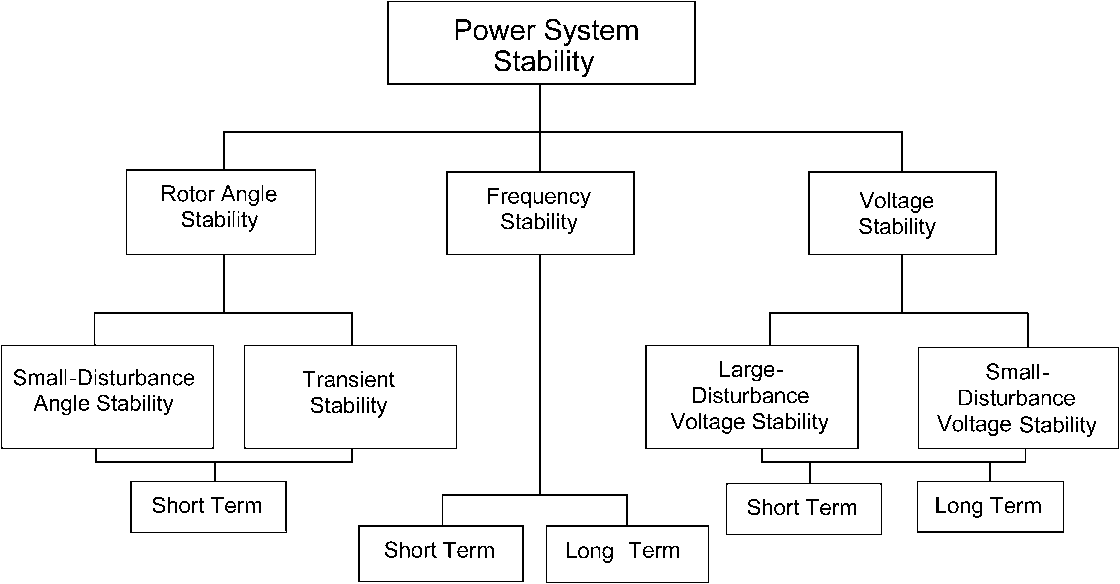
\includegraphics[width=0.9\textwidth]{figurer/Classification_of_power_system_stability}
	\caption{Klassificering af systemstabilitet}
	\label{fig:Overview}
\end{figure}

I dette projekt er det hovedsageligt relevant at undersøge implementeringen af batteriers effekt på nettets frekvensstabilitet og spændingsstabilitet. Dette skyldes at frekvensstabilitet hænger sammen med forholdet mellem produktion og belastning af nettet og spændingsstabilitet hænger sammen med belastningen af nettet, samt kompensering af reaktiv effekt. Rotorvinkelstabilitet er primært relateret til synkron generatorers evne til at forblive synkroniseret med nettet under fejl og vil derfor ikke være et fokus i dette projekt. \\
En forklaring af de stabilitetsproblemer der kan forekomme i forbindelse med frekvensstabilitet og spændingsstabilitet er derfor gennemgået i de følgende afsnit.